\chapter{Doctor Alert with an ESP32}\label{ch:alert}

An alarm helps only if someone can act on it quickly. When the KV260 raises an alarm, an ESP32 on the same breadboard
tells the doctor, who may be in a cabin or another room.

\section{Architecture}

\begin{itemize}
\item \textbf{Board to ESP32:} the board sends one short message per event over the ESP32's USB cable (alarm start,
  updates every 15\,s, escalations, end, patient button). The FPGA's alarm pin (PMOD B1) is also wired to an ESP32
  input as a backup that works even if the board's software stops. The USB cable also powers the ESP32.
\item \textbf{ESP32 to phone:} the ESP32 joins the phone's Wi-Fi hotspot and sends a push notification through the
  ntfy service (iPhone and Android app), and serves a live alarm page on the same network.
\item \textbf{Phone to board:} the doctor's ``On my way'' reaches the ESP32 and is sent back to the board, where the
  dashboard shows it.
\end{itemize}

\section{What the Doctor Sees}

The detector answers ``seizure-like or not''; it was not trained to name a seizure type, so the alert reports only
signs that the front end measures, compared with the minute before the alarm:

\begin{table}[H]
\centering\small
\caption{The signs in the alert.}\label{tab:signs}
\begin{tabularx}{\textwidth}{@{}lLP{50mm}@{}}
\toprule
\textbf{Sign} & \textbf{Shown as} & \textbf{Measured from}\\
\midrule
Heart rate & before and now, NORMAL / HIGH / VERY HIGH & ECG R-peak intervals\\
Shaking & LITTLE / SOME / STRONG & chest accelerometer (or gyroscope)\\
Muscle tension & NORMAL / HIGH & EMG power\\
Brain activity & MILD / HIGH, slow or fast waves & EEG line length and band power\\
Pattern hint & ``motor pattern likely'' or ``little movement'' & movement change\\
\bottomrule
\end{tabularx}
\end{table}

Because the doctor has very little time, the alert is made to be read in about two seconds:

\begin{itemize}
\item \textbf{Notification:} three lines, for example ``SEIZURE Bed 3 / GO TO BED 3 NOW: PROTECT FROM INJURY / Heart
  120 bpm HIGH \textbar{} Shaking STRONG \textbar{} Brain HIGH''.
\item \textbf{Page (Figure~\ref{fig:alertpage}):} status and a running timer; one instruction; ``On my way'' and
  ``Call'' buttons; four colour tiles (red = act, amber = watch, green = normal). The patient's emergency plan, first-aid
  steps and exact numbers are folded below.
\item \textbf{One instruction}, the most urgent first: CHECK BREATHING AND PULSE NOW (heart rate above 150 or below
  40\,bpm, or an unreadable ECG without shaking) $>$ OVER 5 MIN: START EMERGENCY PLAN $>$ OVER 2 MIN: GET EMERGENCY
  PLAN READY $>$ GO TO BED NOW: PROTECT FROM INJURY (strong shaking) $>$ GO TO BED NOW. When it ends: SEIZURE STOPPED:
  CHECK BREATHING, TURN ON SIDE.
\item \textbf{Escalation} at 2 and 5 minutes of alarm, then every minute. Five minutes is the ILAE time point for
  treating a convulsive seizure as status epilepticus; the seizure starts before the alarm, so the real duration is
  longer.
\item \textbf{Reminders} every minute until someone taps ``On my way''; \textbf{clusters} (``2nd seizure this
  hour'') are flagged; no patient names are sent, only a bed name.
\end{itemize}

\begin{figure}[H]
\centering
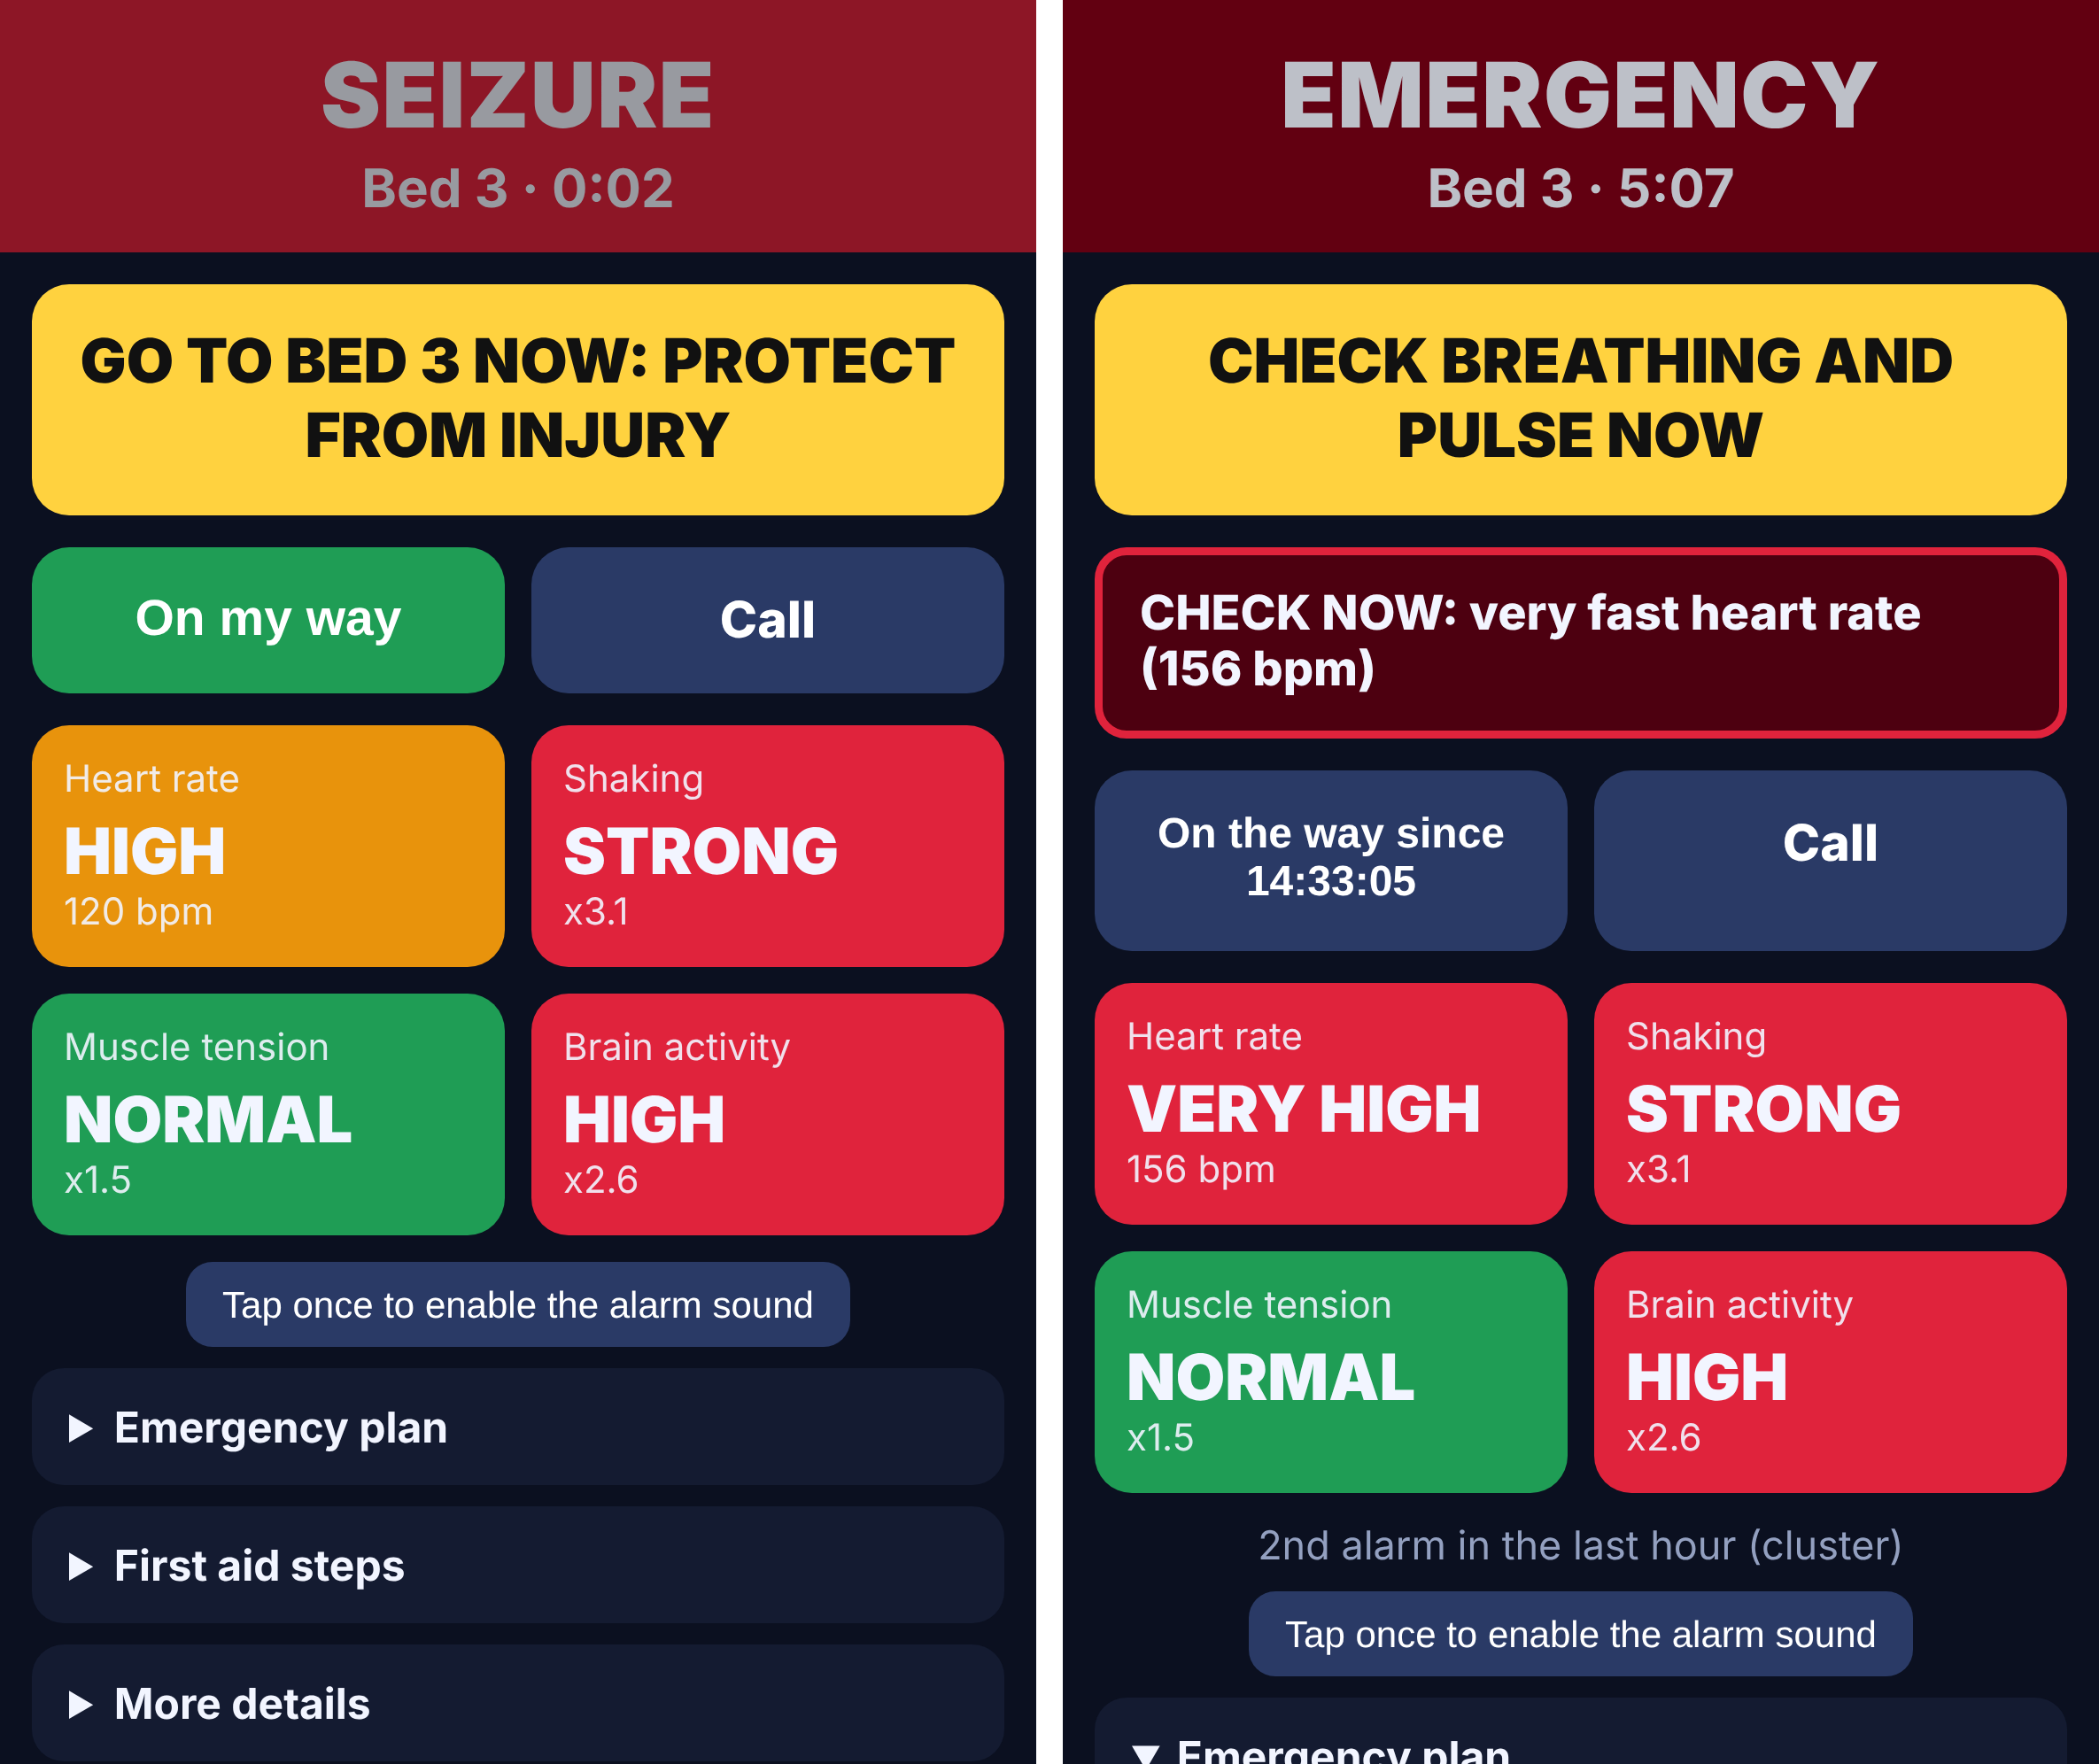
\includegraphics[width=0.9\textwidth]{figures/alert_page.png}
\caption{The doctor's page at a new seizure (left) and in an emergency after 5 minutes (right).}\label{fig:alertpage}
\end{figure}

\section{How Good Is the Pattern Hint?}

We checked the movement-based hint against the doctors' motor / non-motor labels of the 702 seizures of the training
patients only (the test patients were not read):

\begin{itemize}
\item In the first 30\,s, movement rose 4.8-fold (median) in motor seizures and 1.04-fold in non-motor seizures;
  heart rate rose 17\,\% and 8\,\%.
\item A threshold (2.6-fold) chosen on patients 1--48 matched the doctors' label on patients 49--96 in 64\,\% of
  cases (balanced accuracy: 48\,\% of motor and 79\,\% of non-motor seizures). Adding EMG did not help.
\item So the hint is useful but not a diagnosis. The two EEG inputs are one behind-the-ear and one cross-head
  channel chosen per recording, so the alert makes no left/right claim.
\end{itemize}

\section{Testing}

The board side was tested on the emulated board through a virtual serial port: alarm start, updates, end after 30\,s
of quiet, escalation at 2, 5, 6 and 7 minutes (none after the alarm stops), clusters, and the acknowledgement coming
back. The ESP32 program passes a syntax check and the page was rendered at iPhone size. The test on the ESP32 itself,
with a real iPhone, is the next step.
